\documentclass[twoside]{book}

% Packages required by doxygen
\usepackage{fixltx2e}
\usepackage{calc}
\usepackage{doxygen}
\usepackage[export]{adjustbox} % also loads graphicx
\usepackage{graphicx}
\usepackage[utf8]{inputenc}
\usepackage{makeidx}
\usepackage{multicol}
\usepackage{multirow}
\PassOptionsToPackage{warn}{textcomp}
\usepackage{textcomp}
\usepackage[nointegrals]{wasysym}
\usepackage[table]{xcolor}

% Font selection
\usepackage[T1]{fontenc}
\usepackage[scaled=.90]{helvet}
\usepackage{courier}
\usepackage{amssymb}
\usepackage{sectsty}
\renewcommand{\familydefault}{\sfdefault}
\allsectionsfont{%
  \fontseries{bc}\selectfont%
  \color{darkgray}%
}
\renewcommand{\DoxyLabelFont}{%
  \fontseries{bc}\selectfont%
  \color{darkgray}%
}
\newcommand{\+}{\discretionary{\mbox{\scriptsize$\hookleftarrow$}}{}{}}

% Page & text layout
\usepackage{geometry}
\geometry{%
  a4paper,%
  top=2.5cm,%
  bottom=2.5cm,%
  left=2.5cm,%
  right=2.5cm%
}
\tolerance=750
\hfuzz=15pt
\hbadness=750
\setlength{\emergencystretch}{15pt}
\setlength{\parindent}{0cm}
\setlength{\parskip}{3ex plus 2ex minus 2ex}
\makeatletter
\renewcommand{\paragraph}{%
  \@startsection{paragraph}{4}{0ex}{-1.0ex}{1.0ex}{%
    \normalfont\normalsize\bfseries\SS@parafont%
  }%
}
\renewcommand{\subparagraph}{%
  \@startsection{subparagraph}{5}{0ex}{-1.0ex}{1.0ex}{%
    \normalfont\normalsize\bfseries\SS@subparafont%
  }%
}
\makeatother

% Headers & footers
\usepackage{fancyhdr}
\pagestyle{fancyplain}
\fancyhead[LE]{\fancyplain{}{\bfseries\thepage}}
\fancyhead[CE]{\fancyplain{}{}}
\fancyhead[RE]{\fancyplain{}{\bfseries\leftmark}}
\fancyhead[LO]{\fancyplain{}{\bfseries\rightmark}}
\fancyhead[CO]{\fancyplain{}{}}
\fancyhead[RO]{\fancyplain{}{\bfseries\thepage}}
\fancyfoot[LE]{\fancyplain{}{}}
\fancyfoot[CE]{\fancyplain{}{}}
\fancyfoot[RE]{\fancyplain{}{\bfseries\scriptsize Generated by Doxygen }}
\fancyfoot[LO]{\fancyplain{}{\bfseries\scriptsize Generated by Doxygen }}
\fancyfoot[CO]{\fancyplain{}{}}
\fancyfoot[RO]{\fancyplain{}{}}
\renewcommand{\footrulewidth}{0.4pt}
\renewcommand{\chaptermark}[1]{%
  \markboth{#1}{}%
}
\renewcommand{\sectionmark}[1]{%
  \markright{\thesection\ #1}%
}

% Indices & bibliography
\usepackage{natbib}
\usepackage[titles]{tocloft}
\setcounter{tocdepth}{3}
\setcounter{secnumdepth}{5}
\makeindex

% Hyperlinks (required, but should be loaded last)
\usepackage{ifpdf}
\ifpdf
  \usepackage[pdftex,pagebackref=true]{hyperref}
\else
  \usepackage[ps2pdf,pagebackref=true]{hyperref}
\fi
\hypersetup{%
  colorlinks=true,%
  linkcolor=blue,%
  citecolor=blue,%
  unicode%
}

% Custom commands
\newcommand{\clearemptydoublepage}{%
  \newpage{\pagestyle{empty}\cleardoublepage}%
}

\usepackage{caption}
\captionsetup{labelsep=space,justification=centering,font={bf},singlelinecheck=off,skip=4pt,position=top}

%===== C O N T E N T S =====

\begin{document}

% Titlepage & ToC
\hypersetup{pageanchor=false,
             bookmarksnumbered=true,
             pdfencoding=unicode
            }
\pagenumbering{alph}
\begin{titlepage}
\vspace*{7cm}
\begin{center}%
{\Large My Project }\\
\vspace*{1cm}
{\large Generated by Doxygen 1.8.13}\\
\end{center}
\end{titlepage}
\clearemptydoublepage
\pagenumbering{roman}
\tableofcontents
\clearemptydoublepage
\pagenumbering{arabic}
\hypersetup{pageanchor=true}

%--- Begin generated contents ---
\chapter{Class Index}
\section{Class List}
Here are the classes, structs, unions and interfaces with brief descriptions\+:\begin{DoxyCompactList}
\item\contentsline{section}{\hyperlink{structInputData}{Input\+Data} \\*Data structure to store the input data for the coal allocation problem }{\pageref{structInputData}}{}
\item\contentsline{section}{\hyperlink{structState}{State} \\*Represents the state of the problem at any moment during the search }{\pageref{structState}}{}
\end{DoxyCompactList}

\chapter{File Index}
\section{File List}
Here is a list of all documented files with brief descriptions\+:\begin{DoxyCompactList}
\item\contentsline{section}{\hyperlink{problem__solving__by__hill__climbing__search_8c}{problem\+\_\+solving\+\_\+by\+\_\+hill\+\_\+climbing\+\_\+search.\+c} \\*Code for solving the \textquotesingle{}Coal Allocation Problem\textquotesingle{} described in part-\/1 of l2.\+pdf using \textquotesingle{}Hill Climbing Search with Random Restarts\textquotesingle{} }{\pageref{problem__solving__by__hill__climbing__search_8c}}{}
\end{DoxyCompactList}

\chapter{Class Documentation}
\hypertarget{structInputData}{}\section{Input\+Data Struct Reference}
\label{structInputData}\index{Input\+Data@{Input\+Data}}


Data structure to store the input data for the coal allocation problem.  


\subsection*{Public Attributes}
\begin{DoxyCompactItemize}
\item 
int $\ast$$\ast$$\ast$ \hyperlink{structInputData_a1dafb844546b53fd739be0f370676d28}{bid\+\_\+data}
\item 
int $\ast$$\ast$ \hyperlink{structInputData_abb16dba9ad2a732ace6dab1b1c9dec33}{bid\+\_\+data\+\_\+dimensions}
\item 
int $\ast$ \hyperlink{structInputData_a9ae50cca01b0b05cb38c55c328fc19fd}{bid\+\_\+data\+\_\+dimensions\+\_\+dimensions}
\item 
int \hyperlink{structInputData_a8da16cc608de69e099958cfdd162af5a}{num\+\_\+of\+\_\+coal\+\_\+blocks}
\item 
int \hyperlink{structInputData_a8b59f6e5325366bc964a42071441fa90}{num\+\_\+of\+\_\+companies}
\end{DoxyCompactItemize}


\subsection{Detailed Description}
Data structure to store the input data for the coal allocation problem. 

It stores the data as a 3D array. 

\subsection{Member Data Documentation}
\mbox{\Hypertarget{structInputData_a1dafb844546b53fd739be0f370676d28}\label{structInputData_a1dafb844546b53fd739be0f370676d28}} 
\index{Input\+Data@{Input\+Data}!bid\+\_\+data@{bid\+\_\+data}}
\index{bid\+\_\+data@{bid\+\_\+data}!Input\+Data@{Input\+Data}}
\subsubsection{\texorpdfstring{bid\+\_\+data}{bid\_data}}
{\footnotesize\ttfamily int$\ast$$\ast$$\ast$ Input\+Data\+::bid\+\_\+data}

3D array to store the input data. The first dimension corresponds to the company id (cid). The second dimension corresponds to the bids of the particular company set by the first dimension. The first instance in the third dimension is the bid value and the rest corresponds to the block id of the coal. Example usages\+:~\newline
 bid\+\_\+data\mbox{[}i\mbox{]}\+: all the bid data corresponding to the company defined by id i+1 ~\newline
 bid\+\_\+data\mbox{[}i\mbox{]}\mbox{[}j\mbox{]}\+: details of (i+1)-\/th company\textquotesingle{}s j-\/th bid ~\newline
 bid\+\_\+data\mbox{[}i\mbox{]}\mbox{[}j\mbox{]}\mbox{[}0\mbox{]}\+: bid value ~\newline
 bid\+\_\+data\mbox{[}i\mbox{]}\mbox{[}j\mbox{]}\mbox{[}k\mbox{]}\+: block id of the coal (where k$>$0) \mbox{\Hypertarget{structInputData_abb16dba9ad2a732ace6dab1b1c9dec33}\label{structInputData_abb16dba9ad2a732ace6dab1b1c9dec33}} 
\index{Input\+Data@{Input\+Data}!bid\+\_\+data\+\_\+dimensions@{bid\+\_\+data\+\_\+dimensions}}
\index{bid\+\_\+data\+\_\+dimensions@{bid\+\_\+data\+\_\+dimensions}!Input\+Data@{Input\+Data}}
\subsubsection{\texorpdfstring{bid\+\_\+data\+\_\+dimensions}{bid\_data\_dimensions}}
{\footnotesize\ttfamily int$\ast$$\ast$ Input\+Data\+::bid\+\_\+data\+\_\+dimensions}

2D array to keep track of the size of \hyperlink{structInputData_a1dafb844546b53fd739be0f370676d28}{Input\+Data\+::bid\+\_\+data}. It is used since the length of each array in \hyperlink{structInputData_a1dafb844546b53fd739be0f370676d28}{Input\+Data\+::bid\+\_\+data} varies and there are no ways of determining it during runtime using sizeof-\/like functions. Hence, it has to be recorded. \mbox{\Hypertarget{structInputData_a9ae50cca01b0b05cb38c55c328fc19fd}\label{structInputData_a9ae50cca01b0b05cb38c55c328fc19fd}} 
\index{Input\+Data@{Input\+Data}!bid\+\_\+data\+\_\+dimensions\+\_\+dimensions@{bid\+\_\+data\+\_\+dimensions\+\_\+dimensions}}
\index{bid\+\_\+data\+\_\+dimensions\+\_\+dimensions@{bid\+\_\+data\+\_\+dimensions\+\_\+dimensions}!Input\+Data@{Input\+Data}}
\subsubsection{\texorpdfstring{bid\+\_\+data\+\_\+dimensions\+\_\+dimensions}{bid\_data\_dimensions\_dimensions}}
{\footnotesize\ttfamily int$\ast$ Input\+Data\+::bid\+\_\+data\+\_\+dimensions\+\_\+dimensions}

1D array to keep track of the size of \hyperlink{structInputData_abb16dba9ad2a732ace6dab1b1c9dec33}{Input\+Data\+::bid\+\_\+data\+\_\+dimensions}. It is used since the length of each array in \hyperlink{structInputData_abb16dba9ad2a732ace6dab1b1c9dec33}{Input\+Data\+::bid\+\_\+data\+\_\+dimensions} varies and there are no ways of determining it during runtime using sizeof-\/like functions. Hence, it has to be recorded. \mbox{\Hypertarget{structInputData_a8da16cc608de69e099958cfdd162af5a}\label{structInputData_a8da16cc608de69e099958cfdd162af5a}} 
\index{Input\+Data@{Input\+Data}!num\+\_\+of\+\_\+coal\+\_\+blocks@{num\+\_\+of\+\_\+coal\+\_\+blocks}}
\index{num\+\_\+of\+\_\+coal\+\_\+blocks@{num\+\_\+of\+\_\+coal\+\_\+blocks}!Input\+Data@{Input\+Data}}
\subsubsection{\texorpdfstring{num\+\_\+of\+\_\+coal\+\_\+blocks}{num\_of\_coal\_blocks}}
{\footnotesize\ttfamily int Input\+Data\+::num\+\_\+of\+\_\+coal\+\_\+blocks}

The number of coal blocks for auction. \mbox{\Hypertarget{structInputData_a8b59f6e5325366bc964a42071441fa90}\label{structInputData_a8b59f6e5325366bc964a42071441fa90}} 
\index{Input\+Data@{Input\+Data}!num\+\_\+of\+\_\+companies@{num\+\_\+of\+\_\+companies}}
\index{num\+\_\+of\+\_\+companies@{num\+\_\+of\+\_\+companies}!Input\+Data@{Input\+Data}}
\subsubsection{\texorpdfstring{num\+\_\+of\+\_\+companies}{num\_of\_companies}}
{\footnotesize\ttfamily int Input\+Data\+::num\+\_\+of\+\_\+companies}

The number of companies who are participating in the auction. 

The documentation for this struct was generated from the following file\+:\begin{DoxyCompactItemize}
\item 
\hyperlink{problem__solving__by__hill__climbing__search_8c}{problem\+\_\+solving\+\_\+by\+\_\+hill\+\_\+climbing\+\_\+search.\+c}\end{DoxyCompactItemize}

\hypertarget{structState}{}\section{State Struct Reference}
\label{structState}\index{State@{State}}


Represents the state of the problem at any moment during the search.  


\subsection*{Public Attributes}
\begin{DoxyCompactItemize}
\item 
int \hyperlink{structState_aff5c814b2070259023644917cc7bdd2e}{num\+\_\+of\+\_\+companies}
\item 
int \hyperlink{structState_a9d0176a5edaf8f81c9e69bc3e1579f04}{num\+\_\+of\+\_\+coal\+\_\+blocks}
\item 
int $\ast$ \hyperlink{structState_a52cd42ec679f0af76c92ff88d7a079a0}{selected\+\_\+bids\+\_\+from\+\_\+companies}
\item 
int $\ast$ \hyperlink{structState_a9b7fe730b545c321dec2897f8c3c8cbf}{allocated\+\_\+coal\+\_\+blocks}
\end{DoxyCompactItemize}


\subsection{Detailed Description}
Represents the state of the problem at any moment during the search. 

The state at any moment is represented by\+:~\newline
1) \hyperlink{structState_a52cd42ec679f0af76c92ff88d7a079a0}{State\+::selected\+\_\+bids\+\_\+from\+\_\+companies}~\newline
2) \hyperlink{structState_a9b7fe730b545c321dec2897f8c3c8cbf}{State\+::allocated\+\_\+coal\+\_\+blocks} 

\subsection{Member Data Documentation}
\mbox{\Hypertarget{structState_a9b7fe730b545c321dec2897f8c3c8cbf}\label{structState_a9b7fe730b545c321dec2897f8c3c8cbf}} 
\index{State@{State}!allocated\+\_\+coal\+\_\+blocks@{allocated\+\_\+coal\+\_\+blocks}}
\index{allocated\+\_\+coal\+\_\+blocks@{allocated\+\_\+coal\+\_\+blocks}!State@{State}}
\subsubsection{\texorpdfstring{allocated\+\_\+coal\+\_\+blocks}{allocated\_coal\_blocks}}
{\footnotesize\ttfamily int$\ast$ State\+::allocated\+\_\+coal\+\_\+blocks}

Represents the allocation status of the blocks of coal\+: 1) true\+: allocated 2) false\+: not allocated \mbox{\Hypertarget{structState_a9d0176a5edaf8f81c9e69bc3e1579f04}\label{structState_a9d0176a5edaf8f81c9e69bc3e1579f04}} 
\index{State@{State}!num\+\_\+of\+\_\+coal\+\_\+blocks@{num\+\_\+of\+\_\+coal\+\_\+blocks}}
\index{num\+\_\+of\+\_\+coal\+\_\+blocks@{num\+\_\+of\+\_\+coal\+\_\+blocks}!State@{State}}
\subsubsection{\texorpdfstring{num\+\_\+of\+\_\+coal\+\_\+blocks}{num\_of\_coal\_blocks}}
{\footnotesize\ttfamily int State\+::num\+\_\+of\+\_\+coal\+\_\+blocks}

For storing the length of \hyperlink{structState_a9b7fe730b545c321dec2897f8c3c8cbf}{State\+::allocated\+\_\+coal\+\_\+blocks}. Does not change during the search. Defined for convenience. \mbox{\Hypertarget{structState_aff5c814b2070259023644917cc7bdd2e}\label{structState_aff5c814b2070259023644917cc7bdd2e}} 
\index{State@{State}!num\+\_\+of\+\_\+companies@{num\+\_\+of\+\_\+companies}}
\index{num\+\_\+of\+\_\+companies@{num\+\_\+of\+\_\+companies}!State@{State}}
\subsubsection{\texorpdfstring{num\+\_\+of\+\_\+companies}{num\_of\_companies}}
{\footnotesize\ttfamily int State\+::num\+\_\+of\+\_\+companies}

For storing the length of \hyperlink{structState_a52cd42ec679f0af76c92ff88d7a079a0}{State\+::selected\+\_\+bids\+\_\+from\+\_\+companies}. Does not change during the search. Defined for convenience. \mbox{\Hypertarget{structState_a52cd42ec679f0af76c92ff88d7a079a0}\label{structState_a52cd42ec679f0af76c92ff88d7a079a0}} 
\index{State@{State}!selected\+\_\+bids\+\_\+from\+\_\+companies@{selected\+\_\+bids\+\_\+from\+\_\+companies}}
\index{selected\+\_\+bids\+\_\+from\+\_\+companies@{selected\+\_\+bids\+\_\+from\+\_\+companies}!State@{State}}
\subsubsection{\texorpdfstring{selected\+\_\+bids\+\_\+from\+\_\+companies}{selected\_bids\_from\_companies}}
{\footnotesize\ttfamily int$\ast$ State\+::selected\+\_\+bids\+\_\+from\+\_\+companies}

Stores the indices of the selected bids from \hyperlink{structInputData}{Input\+Data}. It stores one bid from the set of bids proposed by a company. The index value corresponding to the bid data in \hyperlink{structInputData_a1dafb844546b53fd739be0f370676d28}{Input\+Data\+::bid\+\_\+data} is stored. A company from which no bid is sleceted has no\+\_\+bid value set at its index. Such a definition was used for the ease of change inside the code of generate\+\_\+successor. 

The documentation for this struct was generated from the following file\+:\begin{DoxyCompactItemize}
\item 
\hyperlink{problem__solving__by__hill__climbing__search_8c}{problem\+\_\+solving\+\_\+by\+\_\+hill\+\_\+climbing\+\_\+search.\+c}\end{DoxyCompactItemize}

\chapter{File Documentation}
\hypertarget{problem__solving__by__hill__climbing__search_8c}{}\section{problem\+\_\+solving\+\_\+by\+\_\+hill\+\_\+climbing\+\_\+search.\+c File Reference}
\label{problem__solving__by__hill__climbing__search_8c}\index{problem\+\_\+solving\+\_\+by\+\_\+hill\+\_\+climbing\+\_\+search.\+c@{problem\+\_\+solving\+\_\+by\+\_\+hill\+\_\+climbing\+\_\+search.\+c}}


Code for solving the \textquotesingle{}Coal Allocation Problem\textquotesingle{} described in part-\/1 of l2.\+pdf using \textquotesingle{}Hill Climbing Search with Random Restarts\textquotesingle{}.  


{\ttfamily \#include $<$stdio.\+h$>$}\newline
{\ttfamily \#include $<$stdlib.\+h$>$}\newline
Include dependency graph for problem\+\_\+solving\+\_\+by\+\_\+hill\+\_\+climbing\+\_\+search.\+c\+:\nopagebreak
\begin{figure}[H]
\begin{center}
\leavevmode
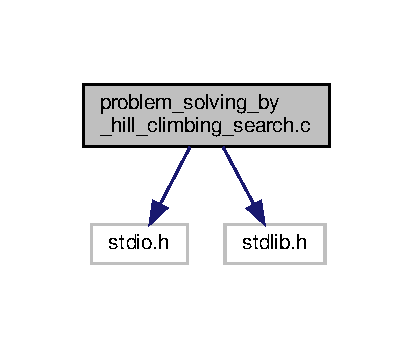
\includegraphics[width=198pt]{problem__solving__by__hill__climbing__search_8c__incl}
\end{center}
\end{figure}
\subsection*{Classes}
\begin{DoxyCompactItemize}
\item 
struct \hyperlink{structState}{State}
\begin{DoxyCompactList}\small\item\em Represents the state of the problem at any moment during the search. \end{DoxyCompactList}\item 
struct \hyperlink{structInputData}{Input\+Data}
\begin{DoxyCompactList}\small\item\em Data structure to store the input data for the coal allocation problem. \end{DoxyCompactList}\end{DoxyCompactItemize}
\subsection*{Macros}
\begin{DoxyCompactItemize}
\item 
\#define \hyperlink{problem__solving__by__hill__climbing__search_8c_a41f9c5fb8b08eb5dc3edce4dcb37fee7}{true}~1
\item 
\#define \hyperlink{problem__solving__by__hill__climbing__search_8c_a65e9886d74aaee76545e83dd09011727}{false}~0
\item 
\#define \hyperlink{problem__solving__by__hill__climbing__search_8c_a262fff7b6a02b30bf9479c7a5e01f909}{no\+\_\+bid}~-\/1
\end{DoxyCompactItemize}
\subsection*{Functions}
\begin{DoxyCompactItemize}
\item 
struct \hyperlink{structState}{State} $\ast$ \hyperlink{problem__solving__by__hill__climbing__search_8c_a81dcbf0d7cbf48b5bb5513cdacf593fc}{create\+\_\+copy\+\_\+state} (struct \hyperlink{structState}{State} $\ast$state)
\begin{DoxyCompactList}\small\item\em Utility function to create a copy of a \hyperlink{structState}{State} object. \end{DoxyCompactList}\item 
\mbox{\Hypertarget{problem__solving__by__hill__climbing__search_8c_accf1874dc9bc755af633b93291382804}\label{problem__solving__by__hill__climbing__search_8c_accf1874dc9bc755af633b93291382804}} 
int {\bfseries cost\+\_\+heuristic} (struct \hyperlink{structState}{State} $\ast$state, struct \hyperlink{structInputData}{Input\+Data} $\ast$input\+\_\+data)
\item 
\mbox{\Hypertarget{problem__solving__by__hill__climbing__search_8c_a207d35ea29548de1a03cb83daa2156a7}\label{problem__solving__by__hill__climbing__search_8c_a207d35ea29548de1a03cb83daa2156a7}} 
int {\bfseries check\+\_\+bid\+\_\+collision} (int $\ast$allocated\+\_\+coal\+\_\+blocks, int $\ast$bid, int bid\+\_\+length)
\item 
struct \hyperlink{structState}{State} $\ast$ \hyperlink{problem__solving__by__hill__climbing__search_8c_a931e0f5e6aee376125af003fab57cfba}{generate\+\_\+successor} (struct \hyperlink{structState}{State} $\ast$old\+\_\+state, struct \hyperlink{structInputData}{Input\+Data} $\ast$input\+\_\+data)
\item 
\mbox{\Hypertarget{problem__solving__by__hill__climbing__search_8c_a90b929de2b481dcb8d65cacdbcb0ad25}\label{problem__solving__by__hill__climbing__search_8c_a90b929de2b481dcb8d65cacdbcb0ad25}} 
struct \hyperlink{structState}{State} $\ast$ {\bfseries find\+\_\+initial\+\_\+state} (struct \hyperlink{structInputData}{Input\+Data} $\ast$input\+\_\+data)
\item 
\mbox{\Hypertarget{problem__solving__by__hill__climbing__search_8c_a62d9c3a87104c1f674b8063912c52337}\label{problem__solving__by__hill__climbing__search_8c_a62d9c3a87104c1f674b8063912c52337}} 
struct \hyperlink{structState}{State} $\ast$ {\bfseries formulate\+\_\+goal} (struct \hyperlink{structInputData}{Input\+Data} $\ast$input\+\_\+data)
\item 
\mbox{\Hypertarget{problem__solving__by__hill__climbing__search_8c_a7db5c37cb88f315f06f893ffb290922b}\label{problem__solving__by__hill__climbing__search_8c_a7db5c37cb88f315f06f893ffb290922b}} 
int {\bfseries is\+\_\+goal\+\_\+state} (struct \hyperlink{structState}{State} $\ast$state, struct \hyperlink{structState}{State} $\ast$goal\+\_\+state)
\item 
struct \hyperlink{structInputData}{Input\+Data} $\ast$ \hyperlink{problem__solving__by__hill__climbing__search_8c_abf96505e915ac91777e34ee4803fd109}{take\+\_\+input} (char file\+\_\+name\mbox{[}$\,$\mbox{]})
\begin{DoxyCompactList}\small\item\em Takes in input from the file name specified. \end{DoxyCompactList}\item 
\mbox{\Hypertarget{problem__solving__by__hill__climbing__search_8c_a66893bf99465548eeebb9316e133daff}\label{problem__solving__by__hill__climbing__search_8c_a66893bf99465548eeebb9316e133daff}} 
void {\bfseries display\+\_\+input\+\_\+data} (struct \hyperlink{structInputData}{Input\+Data} $\ast$input\+\_\+data)
\item 
\mbox{\Hypertarget{problem__solving__by__hill__climbing__search_8c_ad863c528bd134197eb4ec798a0018095}\label{problem__solving__by__hill__climbing__search_8c_ad863c528bd134197eb4ec798a0018095}} 
void {\bfseries display\+\_\+state} (struct \hyperlink{structState}{State} $\ast$state, struct \hyperlink{structInputData}{Input\+Data} $\ast$input\+\_\+data)
\item 
\mbox{\Hypertarget{problem__solving__by__hill__climbing__search_8c_aa3190ec5f3a95333031d02ae42da0341}\label{problem__solving__by__hill__climbing__search_8c_aa3190ec5f3a95333031d02ae42da0341}} 
void {\bfseries deallocate\+\_\+input\+\_\+data} (struct \hyperlink{structInputData}{Input\+Data} $\ast$input\+\_\+data)
\item 
void \hyperlink{problem__solving__by__hill__climbing__search_8c_a501244b2b99bea47cf78b36e87ee9d57}{deallocate\+\_\+state} (struct \hyperlink{structState}{State} $\ast$state)
\begin{DoxyCompactList}\small\item\em Deallocates the memory used by an instance of struct \hyperlink{structState}{State}. \end{DoxyCompactList}\item 
int \hyperlink{problem__solving__by__hill__climbing__search_8c_abf9e6b7e6f15df4b525a2e7705ba3089}{main} (int argc, char const $\ast$argv\mbox{[}$\,$\mbox{]})
\begin{DoxyCompactList}\small\item\em The main function from which all function calls are made. \end{DoxyCompactList}\end{DoxyCompactItemize}


\subsection{Detailed Description}
Code for solving the \textquotesingle{}Coal Allocation Problem\textquotesingle{} described in part-\/1 of l2.\+pdf using \textquotesingle{}Hill Climbing Search with Random Restarts\textquotesingle{}. 

\begin{DoxyAuthor}{Author}
Athul Thaliyachira Reji 
\end{DoxyAuthor}
\begin{DoxyDate}{Date}
16 May 2019 
\end{DoxyDate}


\subsection{Macro Definition Documentation}
\mbox{\Hypertarget{problem__solving__by__hill__climbing__search_8c_a65e9886d74aaee76545e83dd09011727}\label{problem__solving__by__hill__climbing__search_8c_a65e9886d74aaee76545e83dd09011727}} 
\index{problem\+\_\+solving\+\_\+by\+\_\+hill\+\_\+climbing\+\_\+search.\+c@{problem\+\_\+solving\+\_\+by\+\_\+hill\+\_\+climbing\+\_\+search.\+c}!false@{false}}
\index{false@{false}!problem\+\_\+solving\+\_\+by\+\_\+hill\+\_\+climbing\+\_\+search.\+c@{problem\+\_\+solving\+\_\+by\+\_\+hill\+\_\+climbing\+\_\+search.\+c}}
\subsubsection{\texorpdfstring{false}{false}}
{\footnotesize\ttfamily \#define false~0}

For use as boolean false \mbox{\Hypertarget{problem__solving__by__hill__climbing__search_8c_a262fff7b6a02b30bf9479c7a5e01f909}\label{problem__solving__by__hill__climbing__search_8c_a262fff7b6a02b30bf9479c7a5e01f909}} 
\index{problem\+\_\+solving\+\_\+by\+\_\+hill\+\_\+climbing\+\_\+search.\+c@{problem\+\_\+solving\+\_\+by\+\_\+hill\+\_\+climbing\+\_\+search.\+c}!no\+\_\+bid@{no\+\_\+bid}}
\index{no\+\_\+bid@{no\+\_\+bid}!problem\+\_\+solving\+\_\+by\+\_\+hill\+\_\+climbing\+\_\+search.\+c@{problem\+\_\+solving\+\_\+by\+\_\+hill\+\_\+climbing\+\_\+search.\+c}}
\subsubsection{\texorpdfstring{no\+\_\+bid}{no\_bid}}
{\footnotesize\ttfamily \#define no\+\_\+bid~-\/1}

Used in \hyperlink{structState_a52cd42ec679f0af76c92ff88d7a079a0}{State\+::selected\+\_\+bids\+\_\+from\+\_\+companies} at indices where no bid is selected from the company corresponding to that index \mbox{\Hypertarget{problem__solving__by__hill__climbing__search_8c_a41f9c5fb8b08eb5dc3edce4dcb37fee7}\label{problem__solving__by__hill__climbing__search_8c_a41f9c5fb8b08eb5dc3edce4dcb37fee7}} 
\index{problem\+\_\+solving\+\_\+by\+\_\+hill\+\_\+climbing\+\_\+search.\+c@{problem\+\_\+solving\+\_\+by\+\_\+hill\+\_\+climbing\+\_\+search.\+c}!true@{true}}
\index{true@{true}!problem\+\_\+solving\+\_\+by\+\_\+hill\+\_\+climbing\+\_\+search.\+c@{problem\+\_\+solving\+\_\+by\+\_\+hill\+\_\+climbing\+\_\+search.\+c}}
\subsubsection{\texorpdfstring{true}{true}}
{\footnotesize\ttfamily \#define true~1}

$<$ For printf() $<$ For fclose() and scanf() For use as boolean true 

\subsection{Function Documentation}
\mbox{\Hypertarget{problem__solving__by__hill__climbing__search_8c_a81dcbf0d7cbf48b5bb5513cdacf593fc}\label{problem__solving__by__hill__climbing__search_8c_a81dcbf0d7cbf48b5bb5513cdacf593fc}} 
\index{problem\+\_\+solving\+\_\+by\+\_\+hill\+\_\+climbing\+\_\+search.\+c@{problem\+\_\+solving\+\_\+by\+\_\+hill\+\_\+climbing\+\_\+search.\+c}!create\+\_\+copy\+\_\+state@{create\+\_\+copy\+\_\+state}}
\index{create\+\_\+copy\+\_\+state@{create\+\_\+copy\+\_\+state}!problem\+\_\+solving\+\_\+by\+\_\+hill\+\_\+climbing\+\_\+search.\+c@{problem\+\_\+solving\+\_\+by\+\_\+hill\+\_\+climbing\+\_\+search.\+c}}
\subsubsection{\texorpdfstring{create\+\_\+copy\+\_\+state()}{create\_copy\_state()}}
{\footnotesize\ttfamily struct \hyperlink{structState}{State}$\ast$ create\+\_\+copy\+\_\+state (\begin{DoxyParamCaption}\item[{struct \hyperlink{structState}{State} $\ast$}]{state }\end{DoxyParamCaption})}



Utility function to create a copy of a \hyperlink{structState}{State} object. 

There are various places in the program where a \hyperlink{structState}{State} type variable had to be copied. This function is useful in such situations. 
\begin{DoxyParams}{Parameters}
{\em state} & A pointer to an instance of \hyperlink{structState}{State} whose copy is to be made \\
\hline
\end{DoxyParams}
\begin{DoxyReturn}{Returns}
new\+\_\+state A pointer to a copy of state 
\end{DoxyReturn}
\mbox{\Hypertarget{problem__solving__by__hill__climbing__search_8c_a501244b2b99bea47cf78b36e87ee9d57}\label{problem__solving__by__hill__climbing__search_8c_a501244b2b99bea47cf78b36e87ee9d57}} 
\index{problem\+\_\+solving\+\_\+by\+\_\+hill\+\_\+climbing\+\_\+search.\+c@{problem\+\_\+solving\+\_\+by\+\_\+hill\+\_\+climbing\+\_\+search.\+c}!deallocate\+\_\+state@{deallocate\+\_\+state}}
\index{deallocate\+\_\+state@{deallocate\+\_\+state}!problem\+\_\+solving\+\_\+by\+\_\+hill\+\_\+climbing\+\_\+search.\+c@{problem\+\_\+solving\+\_\+by\+\_\+hill\+\_\+climbing\+\_\+search.\+c}}
\subsubsection{\texorpdfstring{deallocate\+\_\+state()}{deallocate\_state()}}
{\footnotesize\ttfamily void deallocate\+\_\+state (\begin{DoxyParamCaption}\item[{struct \hyperlink{structState}{State} $\ast$}]{state }\end{DoxyParamCaption})}



Deallocates the memory used by an instance of struct \hyperlink{structState}{State}. 


\begin{DoxyParams}{Parameters}
{\em state} & The instance of struct \hyperlink{structState}{State} whose memory is to be deallocated \\
\hline
\end{DoxyParams}
\begin{DoxyReturn}{Returns}
void 
\end{DoxyReturn}
\mbox{\Hypertarget{problem__solving__by__hill__climbing__search_8c_a931e0f5e6aee376125af003fab57cfba}\label{problem__solving__by__hill__climbing__search_8c_a931e0f5e6aee376125af003fab57cfba}} 
\index{problem\+\_\+solving\+\_\+by\+\_\+hill\+\_\+climbing\+\_\+search.\+c@{problem\+\_\+solving\+\_\+by\+\_\+hill\+\_\+climbing\+\_\+search.\+c}!generate\+\_\+successor@{generate\+\_\+successor}}
\index{generate\+\_\+successor@{generate\+\_\+successor}!problem\+\_\+solving\+\_\+by\+\_\+hill\+\_\+climbing\+\_\+search.\+c@{problem\+\_\+solving\+\_\+by\+\_\+hill\+\_\+climbing\+\_\+search.\+c}}
\subsubsection{\texorpdfstring{generate\+\_\+successor()}{generate\_successor()}}
{\footnotesize\ttfamily struct \hyperlink{structState}{State}$\ast$ generate\+\_\+successor (\begin{DoxyParamCaption}\item[{struct \hyperlink{structState}{State} $\ast$}]{old\+\_\+state,  }\item[{struct \hyperlink{structInputData}{Input\+Data} $\ast$}]{input\+\_\+data }\end{DoxyParamCaption})}

$<$ The flag is set when a new valid bid is detected from a company while the bids from the remaining companies stays the same \mbox{\Hypertarget{problem__solving__by__hill__climbing__search_8c_abf9e6b7e6f15df4b525a2e7705ba3089}\label{problem__solving__by__hill__climbing__search_8c_abf9e6b7e6f15df4b525a2e7705ba3089}} 
\index{problem\+\_\+solving\+\_\+by\+\_\+hill\+\_\+climbing\+\_\+search.\+c@{problem\+\_\+solving\+\_\+by\+\_\+hill\+\_\+climbing\+\_\+search.\+c}!main@{main}}
\index{main@{main}!problem\+\_\+solving\+\_\+by\+\_\+hill\+\_\+climbing\+\_\+search.\+c@{problem\+\_\+solving\+\_\+by\+\_\+hill\+\_\+climbing\+\_\+search.\+c}}
\subsubsection{\texorpdfstring{main()}{main()}}
{\footnotesize\ttfamily int main (\begin{DoxyParamCaption}\item[{int}]{argc,  }\item[{char const $\ast$}]{argv\mbox{[}$\,$\mbox{]} }\end{DoxyParamCaption})}



The main function from which all function calls are made. 

The main function acts as the problem solving agent. This is because all function calls are made from main -\/ formulate\+\_\+goal, find\+\_\+initial\+\_\+state, and generate\+\_\+successor. This was chosen because of the absence of O\+OP in C.


\begin{DoxyParams}{Parameters}
{\em argc} & The number of command prompt arguments \\
\hline
{\em argv} & The array containing all the command prompt arguments \\
\hline
\end{DoxyParams}
\begin{DoxyReturn}{Returns}
0 
\end{DoxyReturn}
\mbox{\Hypertarget{problem__solving__by__hill__climbing__search_8c_abf96505e915ac91777e34ee4803fd109}\label{problem__solving__by__hill__climbing__search_8c_abf96505e915ac91777e34ee4803fd109}} 
\index{problem\+\_\+solving\+\_\+by\+\_\+hill\+\_\+climbing\+\_\+search.\+c@{problem\+\_\+solving\+\_\+by\+\_\+hill\+\_\+climbing\+\_\+search.\+c}!take\+\_\+input@{take\+\_\+input}}
\index{take\+\_\+input@{take\+\_\+input}!problem\+\_\+solving\+\_\+by\+\_\+hill\+\_\+climbing\+\_\+search.\+c@{problem\+\_\+solving\+\_\+by\+\_\+hill\+\_\+climbing\+\_\+search.\+c}}
\subsubsection{\texorpdfstring{take\+\_\+input()}{take\_input()}}
{\footnotesize\ttfamily struct \hyperlink{structInputData}{Input\+Data}$\ast$ take\+\_\+input (\begin{DoxyParamCaption}\item[{char}]{file\+\_\+name\mbox{[}$\,$\mbox{]} }\end{DoxyParamCaption})}



Takes in input from the file name specified. 

Example of input file -\/ \char`\"{}1.\+txt\char`\"{}. The input is stored in a 3-\/D array. The state is taken as the total revenue from allocating the coal blocks at that instant. The maximum value of the revenue is the sum of max revenue offered by each company since all other combinations will give revenue less than this amount. This maximum value is taken as the goal state. The solution obtained can\textquotesingle{}t reach this value but will be the nearest to it.


\begin{DoxyParams}{Parameters}
{\em file\+\_\+name} & the file to take input from \\
\hline
\end{DoxyParams}
\begin{DoxyReturn}{Returns}
void 
\end{DoxyReturn}

%--- End generated contents ---

% Index
\backmatter
\newpage
\phantomsection
\clearemptydoublepage
\addcontentsline{toc}{chapter}{Index}
\printindex

\end{document}
